\subsection{Additive Manufacturing (AM)\hfill IP}
    \begin{footnotesize}
        \begin{itemize}
            \item \textbf{Kostenvorteil AM:}
            \\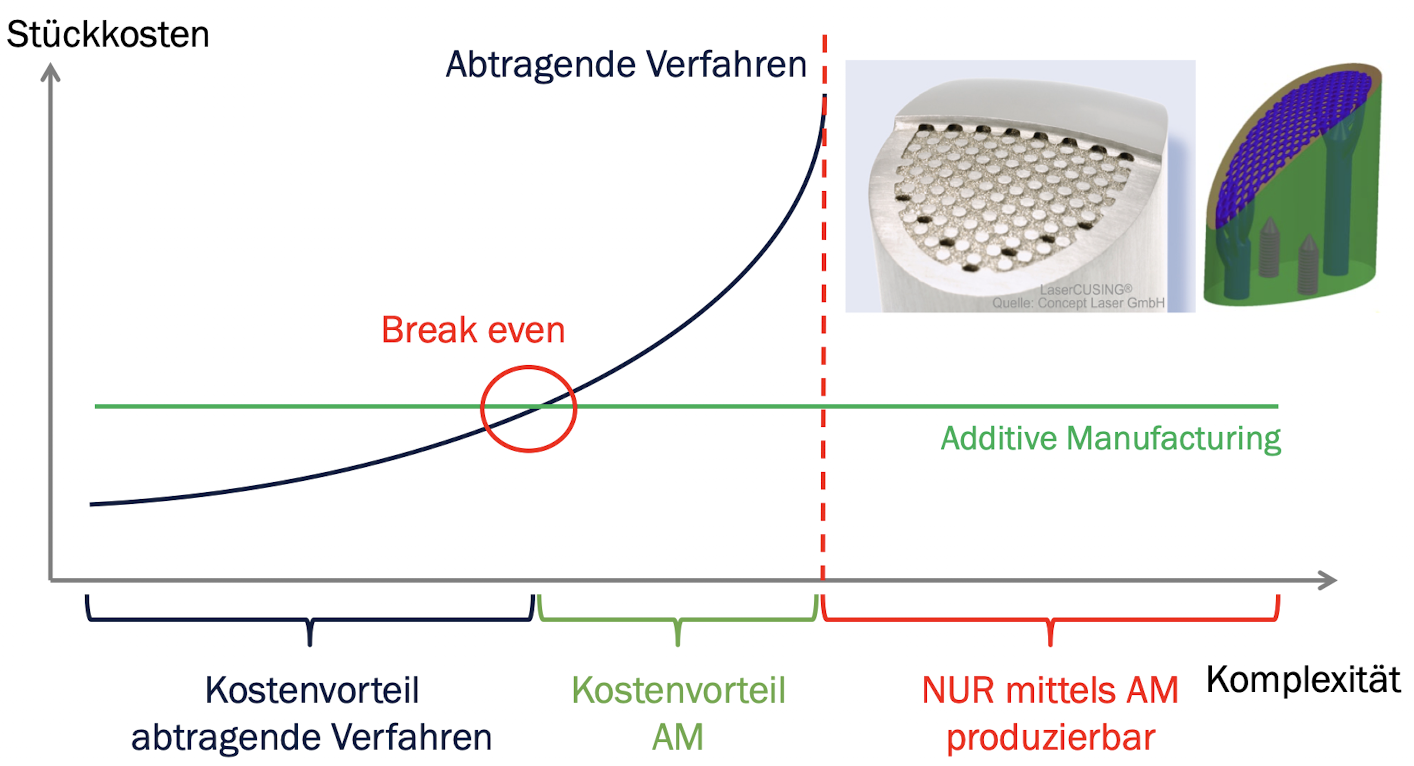
\includegraphics[width = 0.8\linewidth]{src/images/MAEIP_AM}

            \item \textbf{Kostenvorteil Spritzguss:}
            \\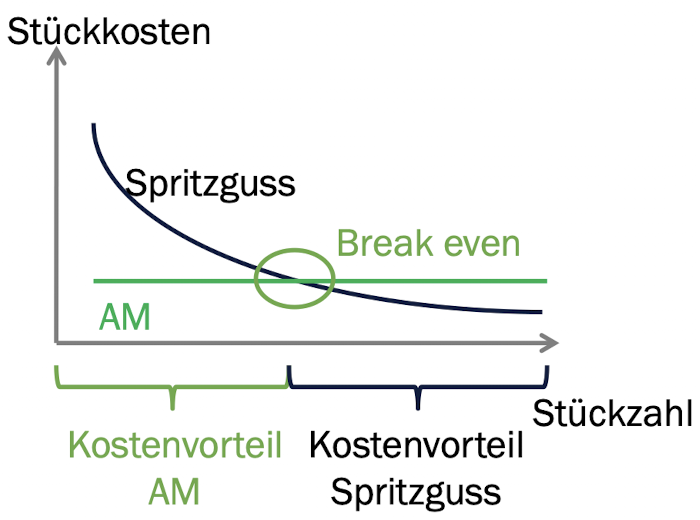
\includegraphics[width = 0.5\linewidth]{src/images/MAEIP_KostenvorteilSpritzguss}
        \end{itemize}
    \end{footnotesize}

    \subsubsection{Stereolithographie \hfill IP}
    \begin{scriptsize}
        Material $\to$ UV-Härtendes Flüssigharz / Übergänge $\to$ mit Hilfe von Stützfunktionen
        \\Ermöglicht Herstellung von \textbf{transparenten Bauteilen} / sehr präzise
    \end{scriptsize}

    \subsubsection{3D-Printing \hfill IP}
    \begin{scriptsize}
        Pulvermaterial $\to$ Kunststoff / Metall / Glas / Keramik / Sand
        \\ mit Kleber zusammengeklebt / mehrstufiger Prozess / im Ofen erhitzt und gehärtet, schrumpft dadurch / \textbf{Farbverläufe} einfach realisierbar
    \end{scriptsize}

    \subsubsection{Fused Deposition Modelling (FDM) \hfill IP}
    \begin{scriptsize}
        Material $\to$ Kunststoff als Draht / Aufschmelzen in Düse / Verwendung von Stützmaterial / Designprototypen / rauhe Oberfläche bei Endprodukt / \textbf{einzelne Schichten und Druckrichtung gut erkennbar}
    \end{scriptsize}

    \subsubsection{Selective Laser Sintering / -Melting \hfill IP}
    \begin{scriptsize}
        Pulvermaterial $\to$ Kunststoff / Metall / Keramik $\to$ Laser schmilzt Material
        \\ \textbf{wird vorzugsweise für metallische Bauteile verwendet}
    \end{scriptsize}